% !TeX spellcheck = fr_FR

% TODO: Replace scan images with clean text where possible

\documentclass[a4paper, 10pt]{report}

\usepackage[french]{babel}
\usepackage[T1]{fontenc}

\usepackage{amsmath, amssymb, amsfonts}

\usepackage{hyperref}
\usepackage{geometry}

\usepackage{xcolor}
\usepackage{graphicx}

\usepackage{fancyhdr}
\usepackage{lastpage}

\usepackage{enumitem}

\geometry{
	a4paper,
	left=25mm,
	right=25mm,
	top=35mm,
	bottom=25mm,
	headsep=5mm,
	headheight=20mm,
}

\definecolor{solution}{HTML}{E5E4E2}
\providecommand{\abs}[1]{\lvert#1\rvert}
\providecommand{\norm}[1]{\lVert#1\rVert}
\DeclareMathOperator{\card}{card}

\begin{document}
	
	\renewcommand{\headrule}{%
		\vspace{-4pt}\hrulefill
		\raisebox{-6.8pt}{\ 
\includegraphics[height=5mm]{../../icon.png}}
		\hrulefill
	}	
	\pagestyle{fancy}
	\fancyhf{}
	
	\fancyhead[L]{\small \slshape Automne 2024}
	\fancyhead[C]{\Large \bfseries Analyse I - Série 03}
	\fancyhead[R]{\small Buff Mathias}
	\fancyfoot[L]{
		\small Source files available at:
		\href{https://github.com/MathiasBuff/bsc-math}
		{github.com/MathiasBuff/bsc-math}
	}
	\fancyfoot[R]{
		\small Page \thepage
		\hspace{1pt} /
		\pageref*{LastPage}
	}
	

	\noindent
	\textbf{Exercice 1.} Soient $E, f \subset \mathbb{R}$ et
	$f : e \to F$ une fonction bijective et monotone. Est-ce que
	$f^{-1}$ est monotone ?
	
	\colorbox{solution}
	{
		\begin{minipage}{0.9\textwidth}
			Comme $f$ est bijective, elle est injective, donc
			strictement monotone.
			
			Sans perte de généralité, pour tou $x, x' \in E,
				x < x' \implies f(x) < f(x')$.\\
			
			Prenons $y, y' \in F$ tels que $y = f(x)$ et $y' = f(x')$.\\
			Comme la fonction inverse de $f$, $f^{-1}$ est bijective
			alors $x = f^{-1}(y)$ et $x' = f^{-1}(y')$.\\
			
			Donc, $f^{-1}(y) < f^{-1}(y') \implies y < y'$ et par
			contraposée, $y \geq y' \implies f^{-1}(y) \geq f^{-1}(y')$.\\
			Par conséquent, $f^{-1}$ est (strictement) monotone.
		\end{minipage}
	}
	
	\vspace{5mm}
	\noindent
	\textbf{Exercice 2.} Les fonctions suivantes sont-elles bien
	définies ? injectives ? surjectives ? bijectives ?
	
	\begin{enumerate}[label=(\roman*)]
		\item $a : \mathbb{N} \to \mathbb{N}\\
			\phantom{a :\ } n \mapsto n + 1$
		%
		\vspace{5pt}
		%
		\item $b : \mathbb{R} \to \mathbb{R}\\
			\phantom{b :\ } x \mapsto 2x$
		%
		\vspace{5pt}
		%
		\item $c : [0, \infty) \to (-\infty, 0]\\
			\phantom{c :\ } x \mapsto x^2$
		%
		\vspace{5pt}
		%
		\item $d : \mathbb{N} \to \{-1, 1\}\\
			\phantom{d :\ } n \mapsto
			\left\{\begin{aligned}
				&1 & &\text{si}\ n\ \text{est pair},\\
				-&1 & &\text{si}\ n\ \text{est impair}
			\end{aligned}\right.$
		%
		\vspace{5pt}
		%
		\item $e : \mathbb{N} \to \{-1, 1\}\\
			\phantom{e :\ } n \mapsto (-1)^n$
	\end{enumerate}
	
	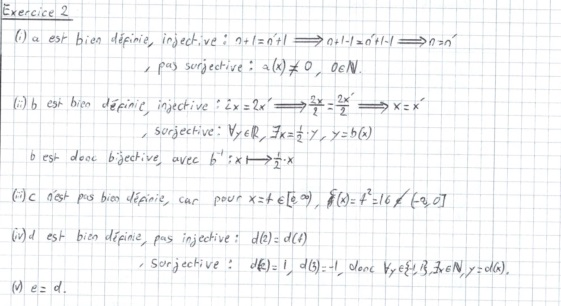
\includegraphics{ex02.jpg}
	
	\vspace{5mm}	
	\noindent
	\textbf{Exercice 3.} Soit $E \subset \mathbb{R}$. Montrer que
	$\sup{E}$, s'il existe, est unique.
	
	\colorbox{solution}
	{
		\begin{minipage}{0.9\textwidth}
			Soit $E \subset \mathbb{R}$, muni d'un supremum noté
			$\sup{E}$.\\
			Supposons un deuxième supremum de $E$, noté $\sup'{E}$.
			Alors $\sup'{E}$ est un majorant de $E$, et comme pour
			tout majorant $M$ de $E$, $\sup{E} \leq M$, alors
			$\sup{E} \leq \sup'{E}$.\\
			
			De la même manière, comme $\sup{E}$ est un majorant de $E$,
			$\sup'{E} \leq \sup{E}$.\\
			Comme $\sup{E} \leq \sup'{E}$ et $\sup'{E} \leq \sup{E}$,
			$\sup{E} = \sup'{E}$.
		\end{minipage}
	}
	
	\newpage
	
	\fancyhf{}
	\renewcommand{\headrule}
	{\rule{\textwidth}{0pt}}
	\fancyfoot[R]{
		\small Page \thepage
		\hspace{1pt} /
		\pageref*{LastPage}
	}
	
	\noindent
	\textbf{Exercice 4.} Trouver le supremum et infimum dans $\mathbb{R}$
	de :
	\begin{enumerate}[label=(\roman*)]
		\item $E = \{\frac{1}{n} + (-1)^n : n \in \mathbb{N}^*\}$
		\item $E = \{x \in \mathbb{R} : 0 \leq x < 1\}$
		\item $E = \{x \in \mathbb{R} : -8 \leq x^3 \leq -1\
			\text{ou}\ 2 \leq x + 1 < 6\}$	
	\end{enumerate}
	Est-ce que ce sont des maximums et des minimums ?
	
	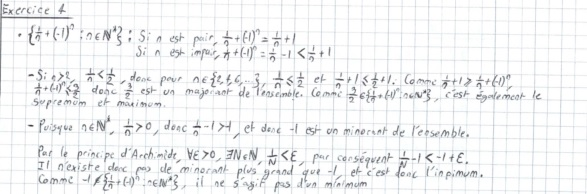
\includegraphics{ex04-p1.jpg}
	
	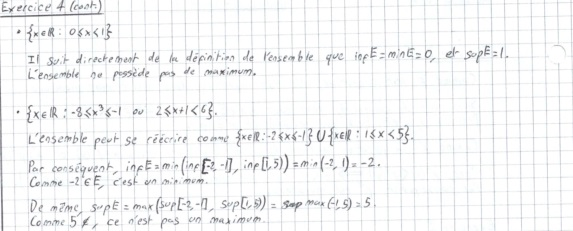
\includegraphics{ex04-p2.jpg}
	
	\vspace{5mm}
	\noindent
	\textbf{Exercice 5.} Déterminer quelles sont les fonctions
	injectives, surjectives, et bijections parmi la liste suivante.
	Justifier vos affirmations.
	\begin{enumerate}[label=(\roman*)]
		\item $f : \mathbb{R} \setminus \{0\} \to
			\mathbb{R} \setminus \{0\}\\
		\phantom{f :\ } x \mapsto \frac{1}{x}$
		%
		\item $g : \mathbb{N} \setminus \{0, 1\} \to \mathbb{N}\\
		\phantom{g :\ } n \mapsto \text{le plus petit nombre premier
			divisant}\ n$
		%
		\item Soit $E$ un ensemble,
		\[\begin{aligned}
			\chi :\ & \mathcal{P}(E) &\to \quad &\{0, 1\}^E\\
			&A &\mapsto \quad &\chi_A
		\end{aligned}\]
		où $\chi_A$ est la fonction caractéristique de l'ensemble $A$.
	\end{enumerate}
	
	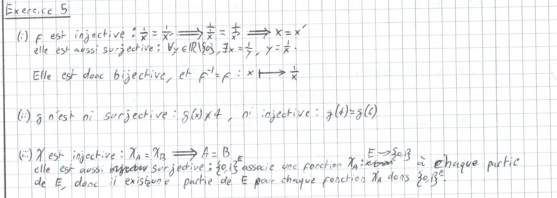
\includegraphics{ex05.jpg}
	
	\vspace{5mm}
	\noindent
	\textbf{Exercice 6.} Déterminer quelles sont les fonctions
	croissantes et décroissantes parmi la liste suivante.
	Justifier vos affirmations.
	\begin{enumerate}[label=(\roman*)]
		\item $\begin{aligned}
			h :\ & \mathbb{R} &&\to &&\mathbb{R}\\
			&x &&\mapsto &&x^2
		\end{aligned} \qquad$ même question avec
		$\qquad \begin{aligned}
			i :\ & [0, \infty) &&\to &&\mathbb{R}\\
			&x &&\mapsto &&x^2
		\end{aligned}$
		%
		\vspace{10pt}
		%
		\item $\begin{aligned}
			\pi :\ & \mathbb{N} &&\to &&\mathbb{N}\\
			&n &&\mapsto &&\pi(n)
		\end{aligned} \qquad$ où $\pi(n)$ est le nombre de nombres
		premiers inférieurs ou égaux à $n$.
	\end{enumerate}
	
	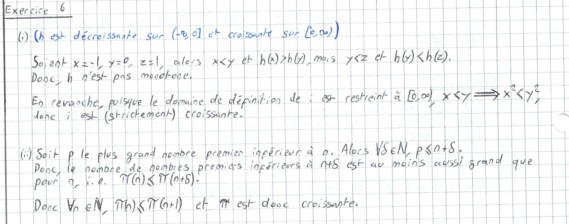
\includegraphics{ex06.jpg}
	
	\vspace{5mm}
	\noindent
	\textbf{Exercice 7.} Soient $E \subset F \subset \mathbb{R}$.
	Montrer que $\sup{E} \leq \sup{F}$ et $\inf{E} \geq \inf{F}$.
	
	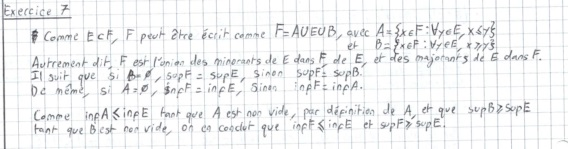
\includegraphics{ex07.jpg}
		
	\newpage
	
	\noindent
	\textbf{Exercice 8.} Soit $f : E \to F$. Montrer que
	\[
		E = \bigcup\limits_{y \in F} f^{-1}(\{y\})
	\]
	
	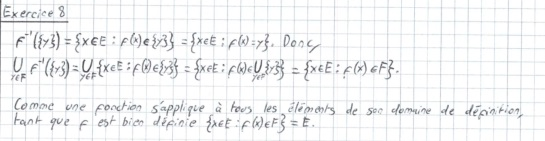
\includegraphics{ex08.jpg}
	
	\vspace{5mm}
	\noindent
	\textbf{Exercice 9.} Soient $f : E \to F$ et $g : F \to G$ deux
	fonctions.
	\begin{enumerate}[label=(\roman*)]
		\item Supposons que $g \circ f$ est injective, est-ce que
		$f$ est injective ? Même question avec $g$ ?
		%
		\item Supposons que $g \circ f$ est surjective, est-ce que
		$f$ est surjective ? Même question avec $g$ ?
		%
		\item Est-ce que $g \circ f$ bijective implique $f$ et $g$
		bijectives ?
	\end{enumerate}	
	Pour chaque question, si la réponse est oui, le prouver.
	Sinon, exhiber un contre-exemple.
	
	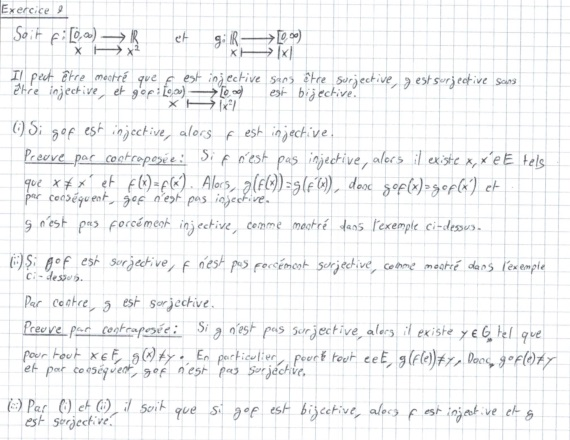
\includegraphics{ex09.jpg}
	
\end{document}
